% Figure 1: the fused cascade. One KICS column (8.2 cm); compile with Tectonic (XeTeX):
%   tectonic figures/method_diagram.tex   -> figures/method_diagram.pdf (PNG for the Word draft: 600 dpi)
% The fusion step is the only accented node (the contribution); the rest is neutral.
\documentclass[border=1pt]{standalone}
\usepackage{fontspec}
\setmainfont{Arial}
\usepackage{amsmath}
\usepackage{tikz}
\usetikzlibrary{positioning,arrows.meta,shapes.geometric}
\definecolor{ours}{HTML}{0072B2}
\definecolor{ink}{HTML}{3A3A3A}
\definecolor{soft}{HTML}{F2F2F2}
\begin{document}
\fontsize{7.5}{9}\selectfont
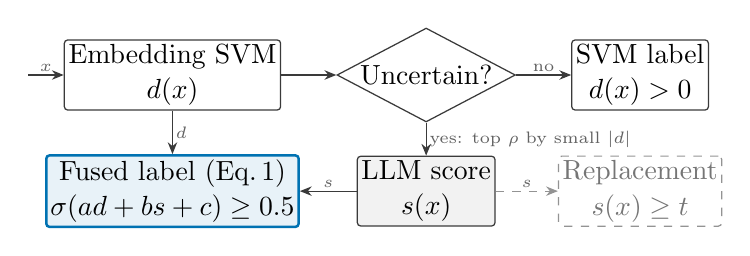
\begin{tikzpicture}[
    node distance=2.6mm and 7mm,
    box/.style={draw=ink, rounded corners=1.2pt, align=center, line width=0.45pt,
                minimum width=15.5mm, minimum height=7.6mm, inner sep=1.5pt},
    llm/.style={box, fill=soft},
    ours/.style={box, draw=ours, fill=ours!9, line width=0.9pt, minimum width=21mm},
    gate/.style={draw=ink, diamond, aspect=1.9, align=center, line width=0.45pt, inner sep=0.6pt},
    flow/.style={-{Stealth[length=1.5mm,width=1.2mm]}, draw=ink, line width=0.45pt},
    lbl/.style={font=\fontsize{6.5}{7.5}\selectfont, text=ink!80, inner sep=1pt},
    base/.style={box, draw=ink!55, dashed, text=ink!70},
    baseflow/.style={flow, draw=ink!55, dashed},
  ]
  \node[box]                       (svm)  {Embedding SVM\\[0.3mm]$d(x)$};
  \node[gate, right=of svm]        (gate) {Uncertain?};
  \node[box, right=of gate]        (keep) {SVM label\\[0.3mm]$d(x)>0$};
  \node[llm, below=4.2mm of gate]  (llm)  {LLM score\\[0.3mm]$s(x)$};
  \node[ours] at (llm -| svm)      (fuse) {Fused label (Eq.\,1)\\[0.3mm]$\sigma(ad+bs+c)\geq 0.5$};
  % the baseline it is compared with, drawn as the road not taken: the replacement cascade drops d
  \node[base] at (llm -| keep)     (repl) {Replacement\\[0.3mm]$s(x)\geq t$};

  \coordinate[left=4.5mm of svm] (in);
  \draw[flow] (in) -- node[lbl, above] {$x$} (svm);
  \draw[flow] (svm) -- (gate);
  \draw[flow] (gate) -- node[lbl, above] {no} (keep);
  % routing step of Sec. 2.2: the call-rate fraction rho of sentences with the smallest |d(x)| go to the LLM
  \draw[flow] (gate) -- node[lbl, right] {yes: top $\rho$ by small $|d|$} (llm);
  \draw[flow] (llm) -- node[lbl, above] {$s$} (fuse);
  \draw[flow] (svm) -- node[lbl, right] {$d$} (fuse);
  \draw[baseflow] (llm) -- node[lbl, above] {$s$} (repl);
\end{tikzpicture}
\end{document}
